\section{Ziel}
\label{sec:Ziel}
Ziel des Versuches ist die Vermessung und anschließende Analyse der Magnetfelder verschiedener Spulen. Betrachtet werden eine "lange" \: Spule, ein Helmholtzspulenpaar und eine 
Toroidspule. Eine Spule wird als \textit{lange Spule} bezeichnet, wenn die Länge der Spule groß gegenüber dem Spulendurchmesser ist.
Es sollen der Verlauf der Magnetfeldstärke der ersten beiden Spulen und die Hysteresekurve des Kernmaterials der Toroidspule untersucht werden.

\section{Theorie}
\label{sec:Theorie}
Bewegen sich Ladungen im Raum, verursachen diese Magnetfelder. So ensteht um einen stromdurchflossenen Leiter ein stationäres Magnetfeld, welches proportional zum Strom 
$I$ des Leiters ist. Die Stärke dieses Magnetfeldes wird mit $\vec{H}$ bezeichnet. Mit der Magnetfeldstärke lässt sich wiederum die magnetische Flussdichte $\vec{B}$ als 
\begin{equation}
    \label{eqn:Flussdichte}
    \vec{B} = \mu_0 \mu_r \vec{H}
\end{equation} 
berechnen. Die Konstante $\mu_0$ wird als \textit{magnetische Feldkonstante} bzw. \textit{Vakuum-Permabilität} bezeichnet. Der zweite Faktor $\mu_r$ ist die 
\textit{relative Permabilität}, welche von dem Material abhängt, in dem sich das Magnetfeld befindet. 

\subsection{Magnetfelder von Spulen}
\label{subsec:Spulen}
Die Flussdichte $\vec{B}$ an der Stelle $\vec{r}$ lässt sich im Vakuum mit dem \textit{Biot-Savartschen Gesetz}
\begin{equation}
    \label{eqn:BiotSavart}
    \symup{d} \vec{B} = \frac{\mu_0 I}{4 \pi}\frac{\symup{d}\vec{s} \times \vec{r}}{r^3}
\end{equation}
durch Integration über den Leiterverlauf berechnen, wobei $r$ den Abstand vom Leiter beschreibt. Für eine runde, geschlossene Leiterschleife ergibt sich so das Magnetfeld
entlang der Symmetrieachse $X$
\begin{equation*}
    \vec{B}(x) = \frac{\mu_0 I}{2} \frac{R^2}{(R^2+x^2)^{3/2}} \cdot {\vec{e}_x}
\end{equation*}
mit dem Radius $R$ der Leiterschleife.
Bei einer langgestreckten, stromdurchflossenen Spule der Länge $l$ ergibt sich durch Überlagerung der Flussdichte von $N$ Leiterschleifen (Windungen) ein homogenes Magnetfeld mit 
Betrag
\begin{equation}
    \label{eqn:LangeSpule}
    B = \mu_r \mu_0 \frac{N I}{l}
\end{equation}
im Inneren der Spule. An den Rändern der Spule gilt dies nicht mehr. 
Um die Randeffekte zu eliminieren, kann die Spule zu einem Ring gebogen werden. Das Magnetfeld des so entstandenen Torus verhält sich im Inneren wie jenes einer langen Spule mit
Länge $l = 2\pi R$. Außerhalb des Torus ist das Magnetfeld konstant 0. 

Ein weiterer Aufbau, mit dem ein homogenes Magnetfeld erzeugt werden kann, ist der des Helmholtzspulenpaares in \autoref{fig:HelmholtzSkizze}.
\begin{figure}{h}{3.5cm}
    \centering
    \caption{Geometrie eines Helmholtzspulenpaares. \cite{v308}}
    \label{fig:HelmholtzSkizze}
    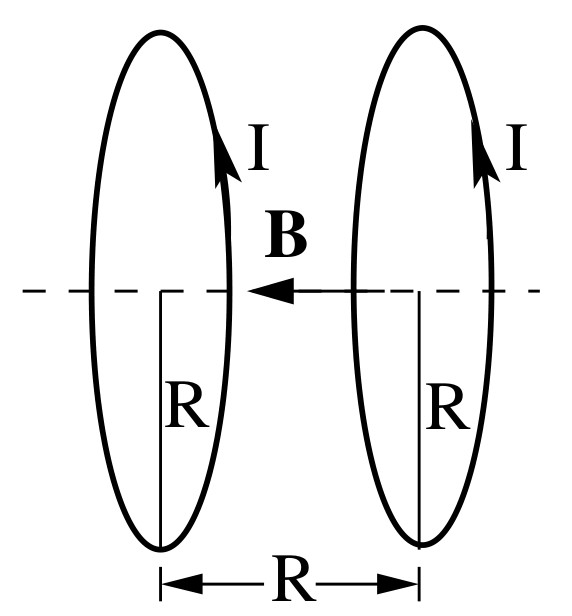
\includegraphics[width=3.5cm]{content/HelmholtzSkizze.jpg}
\end{figure}
Die Spulen sind parallel angeordnet und werden gleichsinnig vom Strom durchflossen. Der Abstand der Spulen sollte dem Spulenradius $R$ entsprechen. Bei einer solchen Anordnung 
ist das Magnetfeld entlang der Symmetrieachse homogen. Falls sich der Abstand $d = 2x$ vom Spulenradius unterscheidet, gilt diese Homogenität nicht mehr. Das Magnetfeld im 
Zentrum eines Spulenpaars mit je einer Windung kann in diesem Fall durch Überlagerung der Felder $B_1$ der einzelnen Spulen als
\begin{equation}
    \label{eqn:Helmholtz}
    B(0) = B_1(x) + B_1(-x) = \frac{\mu_0 I R^2}{(R^2 + x^2)^{3/2}}
\end{equation}
bestimmt werden. Um die Flussdichte für $N$ Windungen pro Spule zu erhalten, kann \autoref{eqn:Helmholtz} mit $N$ multipliziert werden. Die räumliche Ausdehnung
der Spulen wird so nicht berücksichtigt, was jedoch in der Praxis vernachlässigt werden kann. Der Wert der Flussdichte entlang der Symmetrieachse außerhalb des Mittelpunkts lässt sich über
\begin{equation}
    \label{eqn:Helmholtz_theo}
    B(x) = \frac{\mu_0}{2}I R^2 \left(\frac{1}{\left(\left(\frac{d}{2}+x\right)^2 + R^2\right)^{3/2}} + \frac{1}{\left(\left(\frac{d}{2} - x\right)^2 + R^2\right)^{3/2}} \right)
\end{equation}
berechnen \cite{finke92}. Die Variable $x$ beschreibt dabei die Auslenkung vom Mittelpunkt und $d$ den Abstand der Spulen.
Auch der Feldgradient $\frac{\symup{d}B}{\symup{d}x}$ ist im Idealfall in einem relativ großen Bereich vernachlässigbar gering.

\subsection{Magnetisierung ferromagnetischer Stoffe}
\label{subsec:Hysterese}
Wie schon zuvor erwähnt, verhalten sich Magnetfelder in Materie anders als im Vakuum. Die magnetische Flussdichte wird in Materie je nach Art des Mediums
abgeschwächt oder verstärkt. Auf verschiedene Arten des Magnetismus und deren Ursachen wird in \autoref{subsec:VBA} näher eingegangen. Bei ferromagnetischen Stoffen gilt der lineare 
Zusammenhang aus Gleichung \eqref{eqn:Flussdichte} nicht mehr. Für die relative Permabilität $\mu_r$ solcher Stoffe lässt sich kein fester Wert feststellen. Vielmehr wird ein 
komplexerer Zusammenhang deutlich, der sich durch Auftragen der Feldstärke $H$ gegen die Flussdichte $B$ veranschaulichen lässt. Die dadurch entstehende Kurve wird 
\textit{Hysteresekurve} genannt. Ein exemplarischer Verlauf einer Hysteresekurve ist in \autoref{fig:Hysterese} zu sehen.

\begin{figure}
    \centering
    \caption{Schematischer Verlauf einer Hysteresekurve. \cite{v308}}
    \label{fig:Hysterese}
    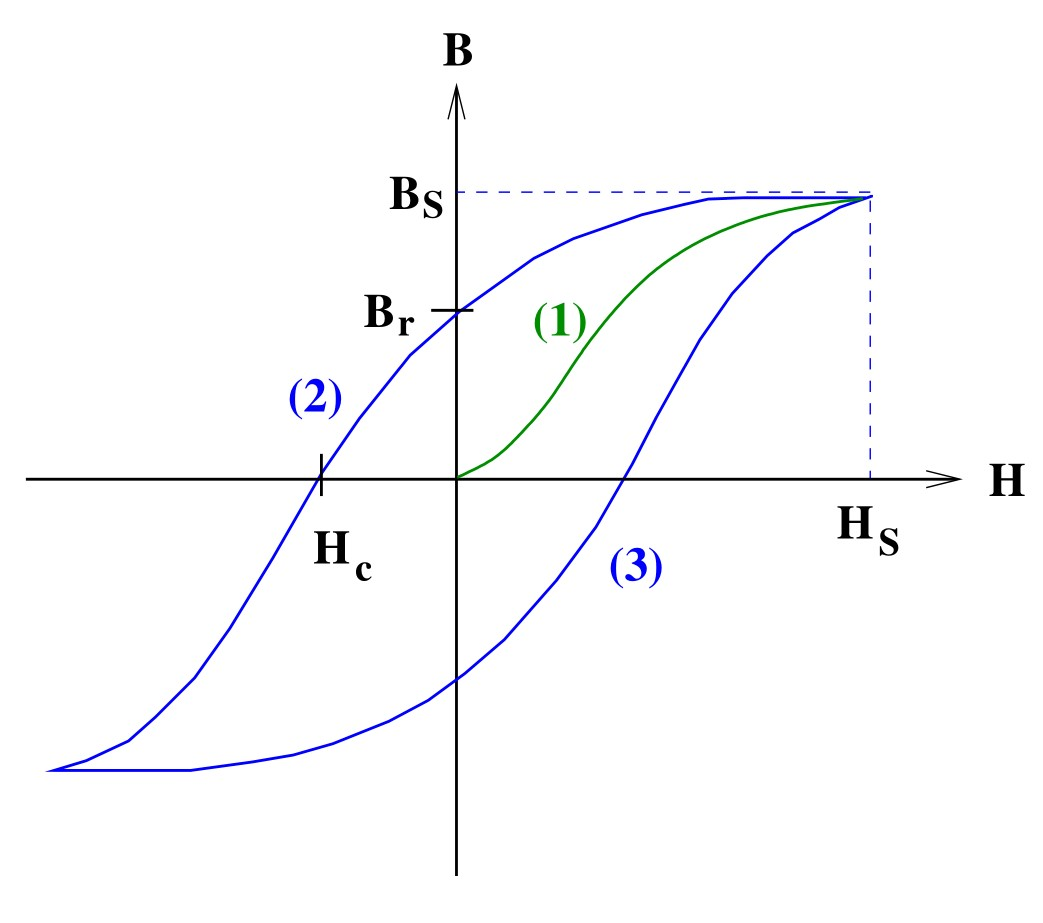
\includegraphics[width=8cm]{content/Hysteresekurve.jpg}
\end{figure}

Wird ein ferromagnetischer Stoff, wie zum Beispiel Eisen, zum ersten Mal einem Magnetfeld ausgesetzt, nimmt die Magnetisierung zuerst zu, bis ein Sättigungswert $B_S$ erreicht wird.
Dieser Kurvenverlauf unterscheidet sich von dem eines bereits magnetisierten Werkstoffes und wird \textit{Neukurve} genannt. In \autoref{fig:Hysterese} ist Diese grün dargestellt. 
Nach Abschalten des externen Magnetfeldes bleibt eine Restmagnetisierung zurück, die mit der Remenanz $B_r \neq 0$ bezeichnet wird. Durch ein Gegenfeld kann die
Magnetisierung des Materials wieder auf 0 eingestellt werden. Die dazu notwendige Feldstärke wird \textit{Koerzitivkraft} $H_c$ genannt. Bei weiterem Erhöhen des externen 
Gegenfeldes wird der negative Wert $-B_S$ des Sättigungswertes erreicht. Wird nun wieder das Gegenfeld verringert und das ursprüngliche Feld erhöht, schließt sich die Kurve 
im Punkt des Sättigungswertes $B_S$. So entsteht ein zum Ursprung symmetrischer Kurvenverlauf.
